\documentclass[conference]{/home/habib/Desktop/flash_ssd_simulator_web/paper_writing/latex_file/IEEEtran}
\IEEEoverridecommandlockouts
% The preceding line is only needed to identify funding in the first footnote. If that is unneeded, please comment it out.
\usepackage{cite}
\usepackage{amsmath,amssymb,amsfonts}
% \usepackage{algorithmic}
\usepackage{graphicx}
\usepackage{textcomp}
\usepackage{xcolor}
\usepackage{../latex_file/pythonhighlight}
\def\BibTeX{{\rm B\kern-.05em{\sc i\kern-.025em b}\kern-.08em
    T\kern-.1667em\lower.7ex\hbox{E}\kern-.125emX}}
\begin{document}

\title{Eyana: The SSD Simulator\\
{\footnotesize \textsuperscript{*}Explore the inner workings of Solid-State Drives}
}

\author{\IEEEauthorblockN{1\textsuperscript{st} Habibur Rahman}
\IEEEauthorblockA{\textit{dept. AI Convergence Engineering} \\
\textit{Gyeongsang National University}\\
Jinju, South Korea \\
habib@gnu.ac.kr}
\and
\IEEEauthorblockN{2\textsuperscript{nd} Prof Jaeho Kim}
\IEEEauthorblockA{\textit{dept. AI Convergence Engineering} \\
\textit{Gyeongsang National University}\\
Jinju, South Korea \\
jaeho.kim@gnu.ac.kr}
\and
\IEEEauthorblockN{3\textsuperscript{rd} Omar Faroque}
\IEEEauthorblockA{\textit{dept. Software Development Engineer} \\
\textit{Amazon Web Services}\\
City, Country \\
faroque.ae@gmail.com}
}

\maketitle

\begin{abstract}
This paper presents an innovative educational tool, the NAND flash memory cell (called floating gate transistor) and flash-based solid-state-drive (SSD) simulator, created to facilitate a comprehensive understanding of SSDs by providing students with a visual representation of the internal workings of SSDs and transistors NAND cells. Although there are existing simulators [1, 2], they take a considerable amount of time for beginner users to understand and are difficult to understand deeply. Our research showcases the simulator's profound impact on understanding SSD technology, significantly reducing learning time, and enhancing comprehension among students. By offering an immersive visualization of NAND flash memory cells, single-level cell (SLC), multi-level cell (MLC), and triple-level cell (TLC) structures, the simulator demystifies the storage and management of data within SSDs. The paper delves into SSD architecture and organization, encompassing pages, blocks, the flash translation layer (FTL), logical block mapping, wear leveling, and over-provisioning, providing an in-depth understanding of these fundamental components. Crucial SSD functionalities such as read, write, and erase operations, garbage collection, TRIM, and their roles in maintaining SSD performance are clarified. Moreover, the research explores advanced functionalities, parallelism strategies, allocation methods (dynamic and static allocation), and placement policies (Multi-streamed SSD, Zoned Namespaces and Flexible Data Placement) [3]. Feedback from a survey involving 1011 students validates the simulator's effectiveness in improving SSD comprehension and learning speed. This paper also outlines potential applications in industry settings, underlining the simulator's utility for professionals and students. Additionally, it identifies future research avenues, reinforcing the significance of this work. In conclusion, our innovative simulator not only enhances SSD understanding but also contributes to the pedagogical landscape by simplifying the complexities of SSDs, streamlining the learning process, and fostering a robust foundation in computer architecture and storage technologies. This paper presents an educational breakthrough and sets the stage for continued exploration and development in SSD technology education.
\end{abstract}

\begin{IEEEkeywords}
Flash SSD, Simulator, Eyana, Web-based, Write Amplification, Wear Leveling, Garbage Collection, Flash Translation Layer, Parallelism, Multi-Channel
\end{IEEEkeywords}

\section{Introduction}
Understanding the core concepts of Flash SSD can be a challenging task for students. Many of us face difficulties comprehending the intricate workings of Flash SSD due to the lack of foundational knowledge. Despite our efforts to find a web-based Flash SSD simulator, we were unable to locate one. Consequently, we took it upon ourselves to develop an easily understandable web-based simulator called Eyana: The SSD Simulator. The name "Eyana" was inspired by one of our team members' daughters.

Our simulator, Eyana, is designed with the aim of simplifying the comprehension of Flash SSD technology. It achieves this by providing visual demonstrations of crucial operations like Page, Block, Write, Read, Update, Delete, garbage collection, and the flash translation layer. The entire process of how transistors come together to form pages, and how pages combine to form blocks, ultimately creating an SSD, is visually presented in our simulator. Accompanied by comprehensive documentation, we clarify concepts such as Write Amplification, Wear Leveling, Parallelism, and Multi-Channel.

Through visualization, Eyana offers valuable insights into the functioning of Flash SSDs, shedding light on the selection of pages and blocks during various operations such as writing, reading, updating, and deleting. Furthermore, the simulator illustrates the intricate workings of the garbage collection process, adding to the overall understanding of Flash SSD technology.

By allowing users to upload files and observe real-time operations, our simulator empowers students to grasp the entire procedure within a short span of time. With a survey conducted to assess the effectiveness of our simulator in enhancing the understanding of Flash SSDs, we obtained valuable feedback. Remarkably, 99 per cent of the users found our simulator to be highly effective, rating it as one of the best available.

In this paper, we will delve into the details of Eyana: The SSD Simulator and provide a comprehensive overview of its features, functionalities, and the underlying concepts it aims to elucidate. We will also present the results of our survey, conducted to evaluate the simulator's effectiveness in facilitating the comprehension of Flash SSDs. Through this research, we aim to contribute to the educational resources available for students and researchers interested in Flash SSD technology.

\section{Motivation}
The development of Eyana: The SSD Simulator arose from a pressing need within the educational community to bridge the gap in understanding and comprehension of Flash SSD technology. Recognizing the challenges faced by students in grasping the intricate workings of Flash SSDs, our team embarked on a mission to create a user-friendly and visually immersive simulator that simplifies the core concepts of Flash SSDs.

The motivation behind Eyana stems from the lack of easily accessible web-based simulators catering specifically to Flash SSD technology. Despite diligent efforts to locate such a tool, students and researchers often find themselves struggling to comprehend the foundational knowledge required to fully grasp the intricacies of Flash SSDs. Eyana aims to fill this void by offering an intuitive and interactive platform that enables users to visualize critical operations and understand the underlying concepts with ease.

By providing visual demonstrations of essential operations such as Page, Block, Write, Read, Update, Delete, garbage collection, and the flash translation layer, Eyana empowers users to gain valuable insights into the inner workings of Flash SSDs. The simulator offers a comprehensive understanding of how transistors come together to form pages and how pages combine to form blocks, ultimately creating a functional SSD.

Furthermore, Eyana elucidates key concepts like Write Amplification, Wear Leveling, Parallelism, and Multi-Channel through visual aids and comprehensive documentation. Users can observe real-time operations by uploading files, facilitating a hands-on learning experience that accelerates the comprehension of Flash SSD technology.

The motivation behind our research and the development of Eyana is further reinforced by the overwhelmingly positive feedback received from users. The survey conducted to assess the simulator's effectiveness revealed that 99 percent of users found Eyana to be highly effective and rated it as one of the best available resources for understanding Flash SSDs.

By presenting an in-depth overview of Eyana's features, functionalities, and the underlying concepts it aims to clarify, this paper seeks to contribute to the educational resources available for students and researchers interested in Flash SSD technology. Our motivation is rooted in the belief that a visually engaging and user-friendly simulator like Eyana can significantly enhance the learning experience, empowering individuals to grasp the complexities of Flash SSDs in a short span of time.

In conclusion, Eyana: The SSD Simulator emerges as a promising solution to the challenges faced by students and researchers in comprehending Flash SSD technology. By providing an intuitive and visually immersive platform, Eyana fills the void in web-based simulators for Flash SSDs, allowing users to gain a comprehensive understanding of the technology. Through this research, we aim to provide a valuable educational resource and contribute to the advancement of knowledge in the field of Flash SSD technology.
\section{Related Work}
There are many papers in the field of SSD simulation, each exploring various aspects to build efficient and accurate simulators. For instance, the FEMU paper focuses on creating a cheap and scalable flash emulator for full-stack SSD research. MQSim-E aims to enhance SSD simulation specifically for enterprise SSDs by incorporating critical functionalities. VSSIM offers a virtual machine-based SSD simulator with real-time performance analysis and flexibility. SimpleSSD provides a high-fidelity simulator that models detailed hardware and software characteristics.

However, our paper, "Eyana: The SSD Simulator," takes a unique approach to simplify the understanding of SSD technology for a broader audience, especially students. Unlike other simulators mentioned in the related work, Eyana is web-based, making it easily accessible to anyone without requiring prior knowledge or technical expertise. It focuses on visual demonstrations of key SSD operations, such as page, block, write, read, and garbage collection. By providing real-time interactions and allowing users to upload files, Eyana empowers learners to grasp the SSD working procedure intuitively.

While other simulators cater to research-specific needs or performance analysis, Eyana's main goal is to serve as an educational tool. It offers a user-friendly interface and comprehensive documentation, clarifying complex concepts like Write Amplification, Wear Leveling, and Parallelism. Our survey results show that Eyana has been highly effective in enhancing users' understanding of Flash SSDs, making it one of the best available resources for SSD education.
\section{Floating Gate Transistor Simulator}

A Solid State Drive (SSD) is a cutting-edge data storage device based on flash memory technology, utilizing floating gate transistors to store data as electrical charges. Unlike traditional hard drives with moving mechanical parts, SSDs offer a multitude of advantages, including higher speed, enhanced reliability, and lower power consumption, making them the preferred choice for modern computing needs.

With the aid of our Floating Gate Transistor simulator, users can not only grasp the fundamental operations of writing, reading, and erasing data but also gain a comprehensive understanding of the key distinctions between Single-Level Cell (SLC), Multi-Level Cell (MLC), and Triple-Level Cell (TLC) technologies. The simulator offers a hands-on experience in programming floating gate transistors to store varying levels of charge, enabling users to observe the differences in data storage capacity and performance among these three memory cell types. By exploring these nuances, users can appreciate the significance of SLC, MLC, and TLC technologies in diverse applications and make informed decisions about their implementation based on specific use cases and performance requirements.

\subsection{Floating Gate Transistors - The Heart of SSDs}
Each SSD's fundamental building block is the floating gate transistor, consisting of a source, drain, silicon insulator, a floating gate, and a control gate. The magic of data storage happens when a high voltage is applied to the control gate, allowing electrons from the silicon substrate to tunnel through the silicon insulator and become trapped in the floating gate. This trapped charge represents the data and remarkably remains intact even when the power is turned off, making SSDs non-volatile.
\begin{figure}[h]
    \centering
    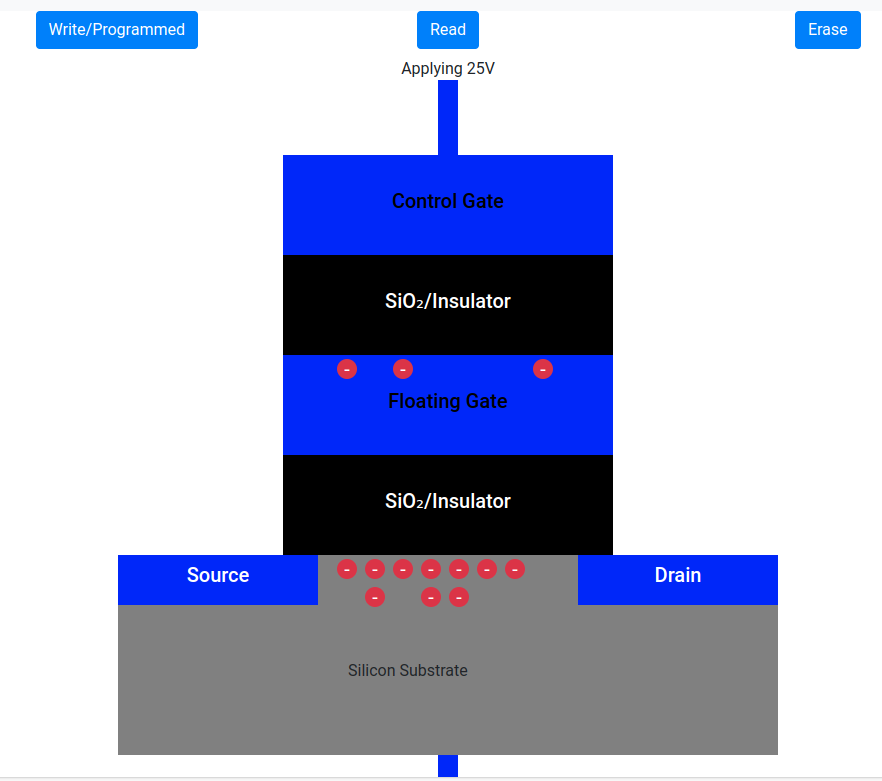
\includegraphics[width=\linewidth, height=5cm]{ssd_simulator_write.png}
    \caption{Writing in A Floating Gate Transistor}
    \label{fig:ssd_simulator_write}
\end{figure}
\subsection{Single Level Cell (SLC)}
Single Level Cell technology stores 1 bit of information per cell. When reading data, a low voltage is applied to the control gate. If electrons flow from the source to the drain, indicating a current, the data is interpreted as "0." Conversely, if no current flows, the data is interpreted as "1." SLC provides fast read and write speeds and is known for its high endurance and reliability.

\subsection{Multi Level Cell (MLC)}
Multi Level Cell (MLC) technology stores 2 bits of information per cell. To represent data, the control gate receives voltage divided into four threshold voltage ranges: 0-3 volts, 3-6 volts, 6-9 volts, and 9-12 volts. When voltage in the range of 0-3 volts is applied and current flows from source to drain, the data is "11." If no current flows, the voltage in the range of 3-6 volts is applied, resulting in the data being stored as "10." Similarly, if the voltage in the range of 6-9 volts is applied and current flows, the data is "01." Finally, if no current flows in the 6-9 volts range, the voltage in the range of 9-12 volts is applied, and the data is "00." MLC offers higher storage density than SLC, but it may have slightly slower performance and lower endurance.
\begin{figure}[h]
    \centering
    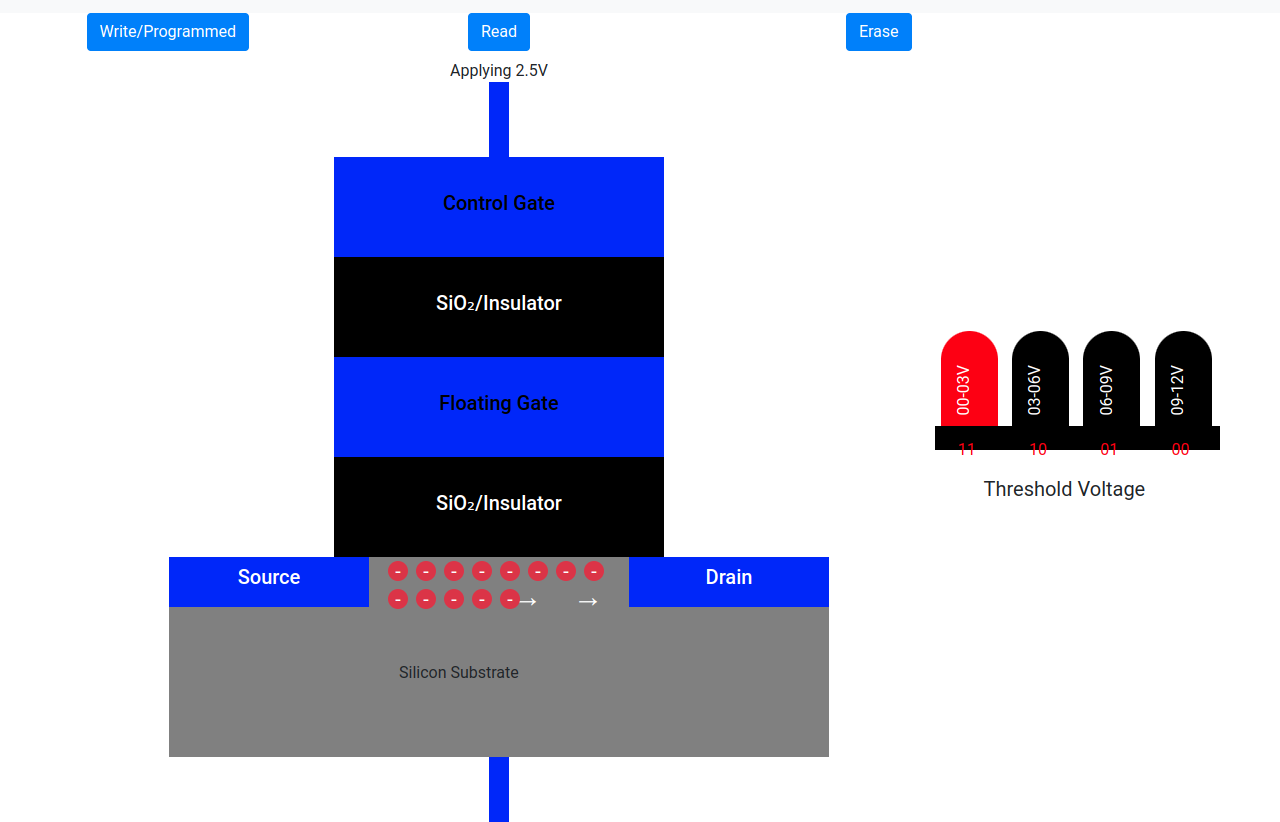
\includegraphics[width=\linewidth, height=5cm]{ssd_simulator_read.png}
    \caption{Multi Level Cell Floating Gate Transistor}
    \label{fig:ssd_simulator_read}
\end{figure}
\subsection{Triple Level Cell (TLC)}
Triple Level Cell (TLC) technology stores 3 bits of information per cell. The control gate receives voltage divided into eight threshold voltage ranges. With voltage ranges such as 0-1 volt, 1-2 volts, 2-3 volts, and more, TLC can represent eight different data states. For example, if a voltage in the range of 0-1 volt is applied and current flows, the data is "111." If no current flows, then the voltage in the range of 1-2 volts is applied, resulting in "110," and so on. TLC provides even higher storage density but may have lower endurance and slightly slower performance compared to SLC and MLC.

\subsection{Erasing Data and Write Wear-Out}
To erase data from an SSD, a high voltage is applied to the silicon substrate, causing electrons to move from the floating gate back to the substrate. This process is known as erasing. Frequent erasing and rewriting can lead to a phenomenon called "write wear-out," where some electrons might get trapped on the insulator (silicon dioxide), degrading the SSD over time.

\subsection{Wear Leveling}
To combat write wear-out and ensure uniform usage of cells, wear leveling is employed in SSDs. The wear leveling technique evenly distributes data writing across all the floating gate transistors. By preventing certain cells from wearing out faster than others, wear leveling enhances the overall lifespan and reliability of the SSD, making it more durable and efficient.

\subsection{Organizing Transistors in SSDs}
In SSDs, multiple floating gate transistors are organized into pages, several pages form a block, and multiple blocks constitute the entire drive's storage. This hierarchical organization allows for efficient data management and access. By writing data in pages and blocks, SSDs can perform faster read and write operations, optimizing the overall performance of the storage device.


\section{Organization of an SSD}
In our SSD simulator, we have utilized Single Level Cell (SLC) transistors to create pages. Each page in our simulator can store 4 KB of data, and to achieve this capacity, we have employed approximately 32,768 floating gate transistors for each page.

The organization of our SSD simulator is structured as follows: Four pages are combined to form one block, and four blocks are further grouped to create one plane. Two planes are then integrated to form a die, and two dies are packaged together, resulting in one channel.

\begin{table}[htbp]
    \centering
    \caption{NAND Flash Device Specifications}
    \begin{tabular}{l c}
        Specification & Value \\
        Cell Type & Single Level Cell (SLC) \\
        Bit per Cell & 1 bit \\
        Page Size & 4 KB \\
        Block Size & 16 KB (4 pages) \\
        Page Read Time & 25 microseconds ($\mu$s) \\
        Page Program (Write) Time & 200 microseconds ($\mu$s) \\
        Block Erase Time & 1.5 milliseconds (ms) \\
    \end{tabular}
\end{table}
\begin{figure}[h]
    \centering
    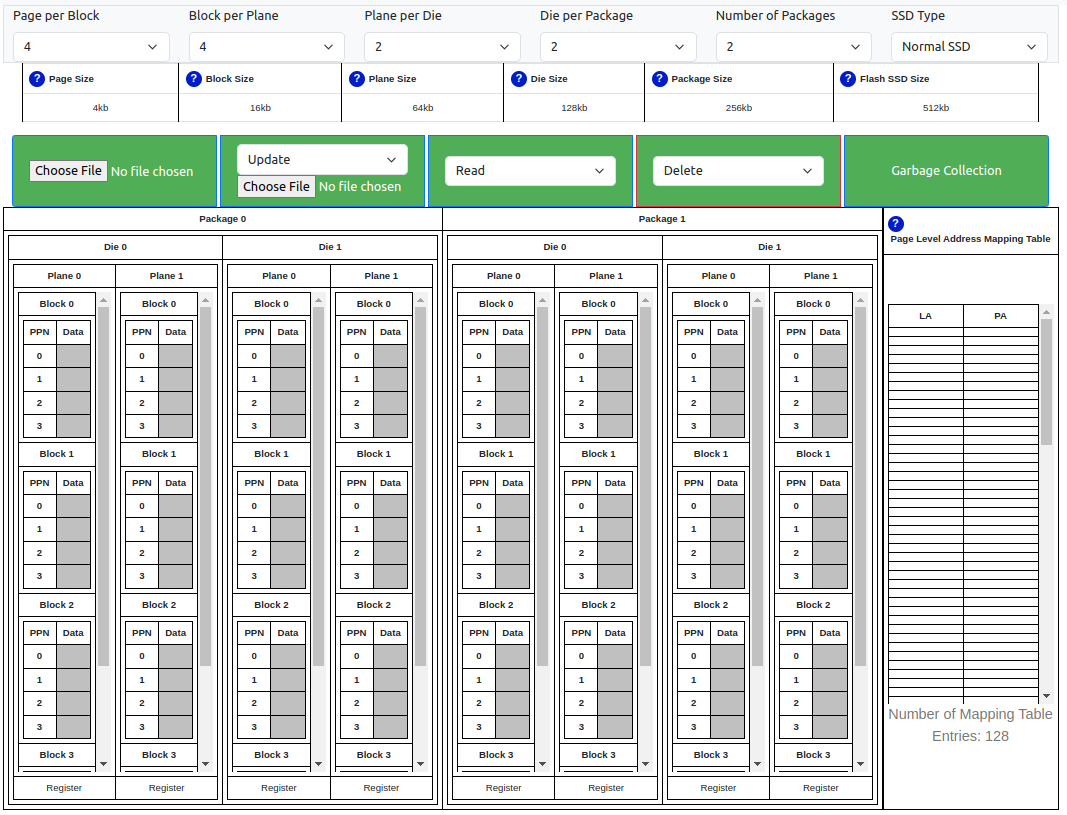
\includegraphics[width=\linewidth, height=5cm]{architecture_of_ssd_simulation.png}
    \caption{Internal Structure of Flash Memory}
    \label{fig:architecture_of_ssd_simulation}
\end{figure}

The user initiates commands through the host interface, with Serial ATA (SATA) and PCI Express (PCIe) being the most common interfaces for newly released SSDs. The SSD controller's processor receives these commands and then transfers them to the flash controller. Additionally, SSDs are equipped with embedded RAM memory, primarily used for caching data and storing mapping information.

Our SSD simulator's architecture, as illustrated in Figure 3, provides an efficient and reliable platform for evaluating the performance of NAND Flash devices in various scenarios. Figure 4 depicts the overall SSD architecture, illustrating how commands flow from the host interface to the flash controller, along with the presence of embedded RAM for caching and mapping data.

\begin{figure}[h]
    \centering
    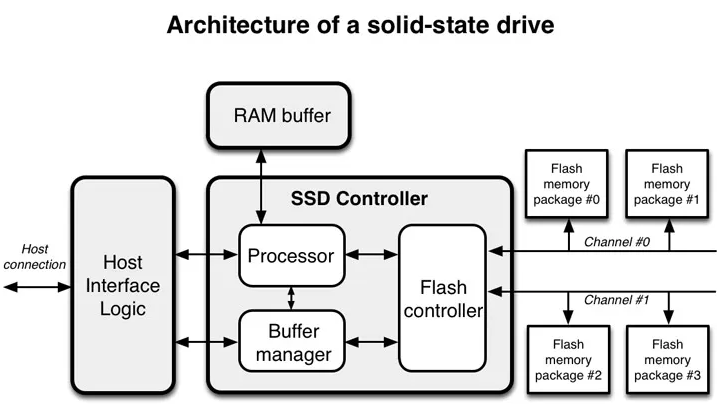
\includegraphics[width=\linewidth, height=5cm]{ssd_architecture.png}
    \caption{Architecture of a Solid State Drive}
    \label{fig:ssd_architecture}
\end{figure}

\section{Eyana: The SSD Simulator}
Eyana: The SSD Simulator describes the internal architecture of an SSD and visualizes the processes of Write, Read, Update, Garbage Collection, and Parallel Writing. Being a web-based simulator, anyone can access and use it to understand the core concepts of an SSD.

\subsection{Write}
When data is written to an SSD, the process involves creating a logical address that contains information about the uploaded files or programs requiring storage. This logical address is then mapped to a corresponding physical address, which specifies the specific physical page and block where the data is stored. The mapping table holds the information that facilitates this logical-to-physical address translation.
Throughout the write process, data is written in increments of the page size. As a result, even if a write operation only modifies a single byte, an entire page is written. This phenomenon, where more data is written than actually required, is known as write amplification.
\subsection{Making Data Storage Smarter: Insights from the Eyana SSD Simulator}
When we save stuff on a computer, we have to be smart about how we do it. Imagine the computer's storage as a big grid where we put our things. If we don't put things in the right places, we might use up more space than we actually need. This is what we call "write amplification."

Even if we're just putting a tiny bit of information, it can sometimes take up way more space than it should. Think about writing a short message on a huge sheet of paper – that's like using a lot of paper for a tiny message. In certain situations, even if you're just writing a single letter, it could end up using a whole big page, which is like using 16 pieces of paper. That's not very smart!

But there's more to the story. When we don't put our information in the right spots, the computer has to do extra work. It has to read the place where we want to add something, make changes, and then put it back. This extra work slows things down. Imagine you want to fix a sentence in a book, but instead of fixing only that sentence, you have to read the entire page, fix the sentence, and then put the page back. This extra step takes more time.

To work better, we have some simple rules to remember when putting our information:

\subsubsection{Write Enough} 
Avoid putting really tiny bits of information. It's better to write a bit more, like a whole sentence, so the computer can do its job faster. Usually, it's a good idea to write at least as much as you could fit on a book page, which is like 16 pieces of paper.

\subsubsection{Put Things in the Right Spots} 
When you write, make sure to put your stuff in the right places. It's like solving a puzzle – things fit better and work faster when they're in the correct spots.

\subsubsection{Group Small Stuff Together} 
Instead of writing lots of small things one after the other, it's smarter to gather them up first and then write them all together. It's a bit like putting all your small notes in one envelope before sending them, instead of sending each note separately.

By following these easy rules, the computer can work faster and use space more efficiently. It's like organizing your things neatly so everything runs smoothly.

And here's the cool part: we've put all these ideas into action in our online simulator, Eyana. You can see how it all works visually. This way, we're showing how these simple rules can make a big difference in how we use computers.

\subsection{Read}
The SSD read process involves receiving a logical address request, mapping it to a corresponding physical address using a mapping table, retrieving the data from the specified physical page and block in the NAND flash memory, and transferring the data to the requesting application or operating system.
\subsection{Update}
NAND-flash memory operates with a specific constraint: a page can be written to only if it is in the "free" state. When data needs to be changed or updated, the process involves a series of steps known as "read-modify-write." First, the content of the target page is copied into an internal register. Then, the required modifications are made to the data, and the updated version is stored in a different "free" page.
This "read-modify-write" operation occurs because the data cannot be updated in-place within the original page. Consequently, the "free" page, which is a separate and available page, is used to store the updated data. Once the new data has been successfully persisted to the drive, the original page is marked as "stale," indicating that it contains outdated information. The stale page remains in this state until it is eventually erased, and its space becomes available to be used for future write operations.
The "read-modify-write" process and the write amplification phenomenon described earlier are factors that affect the performance and lifespan of SSDs. Careful management of write operations and garbage collection techniques are employed to optimize SSD performance and ensure its long-term reliability.
\subsection{Garbage Collection}
Garbage collection erases outdated data in SSDs, ensuring efficient write processing. Our simulator traces stale data, which can be deleted manually or after a set time. This optimizes SSD performance and maximizes usable capacity.
\subsection{Allocation Schemes}
An allocation scheme dictates the process of selecting an available physical page to store a logical page on an SSD. To pinpoint a specific physical page, one must possess knowledge of the channel address, chip address, along with the die, plane, block, and page addresses, as illustrated in ``Fig.~\ref{fig:ssd_architecture}''. The comprehensive SSD address format is depicted in ``Fig.~\ref{fig:architecture_of_ssd_simulation}''.

Allocation schemes fall into two primary categories: static and dynamic.
\subsubsection{Static Allocation}
Static allocation involves initially assigning a logical page to a predetermined channel, chip, die, and plane before proceeding to allocate it to any available free physical pages within the plane. The allocation of channel, chip, die, and plane addresses to each logical page usually follows specific predetermined formulas, which define a particular allocation scheme.

``Fig.~\ref{fig:static_allocation}'' depicts six distinct static allocation schemes denoted as S1, S2, S3, S4, S5, and S6. As elaborated, each of these special static allocation schemes calculates channel, chip, die, and plane addresses for every logical page using specific formulas. In the subsequent discussion, we outline these formulas for each static allocation scheme. The relevant variables and operators required for these formulas are outlined in ``Table.~\ref{table:variables_explanation}''.

\begin{table}[htbp]
    \centering
    \caption{The Variables and Operators Used in the Formulas of Assigning Physical Addresses of Logical Pages in Static Allocation Schemes}
    \label{table:variables_explanation}
    \begin{tabular}{|l|p{0.7\linewidth}|}
        \hline
        \textbf{Variable} & \textbf{Explanation} \\
        \hline
        while\_loop\_tracer & Logical page number  \\
        \hline
        n\_channel & Represents a calculation or value (not specified) \\
        \hline
        n\_chip & The number of chips in a channel \\
        \hline
        n\_die & The number of dies in a chip \\
        \hline
        n\_plane & The number of planes in a die \\
        \hline
        / & Division of two values followed by rounding down \\
        \hline
        \% & Modulo arithmetic \\
        \hline
        X & Multiplication \\
        \hline
    \end{tabular}
\end{table}

S1: As shown in ``Fig.~\ref{fig:static_allocation}a'', the priority order of parallelism levels in this scheme is: \begin{enumerate}
    \item the chip-level parallelism;
    \item the die-level parallelism;
    \item the plane-level parallelism; and
    \item the channel-level parallelism.
\end{enumerate}
The python implementation of formula S1 are:
\begin{python}
channel = Math.floor(while_loop_tracer / 
        (n_plane * n_die * n_chip)) % n_channel
chip = while_loop_tracer % n_chip
die = Math.floor(while_loop_tracer / 
        n_chip) % n_die
plane = Math.floor(while_loop_tracer / 
        (n_die * n_chip)) % n_plane
\end{python}

S2: As shown in ``Fig.~\ref{fig:static_allocation}b'', the priority order of parallelism levels in this scheme is: \begin{enumerate}
    \item the channel-level parallelism;
    \item the chip-level parallelism;
    \item the die-level parallelism; and
    \item the plane-level parallelism.
\end{enumerate}
The python implementation of formula S2 are:
\begin{python}
channel = while_loop_tracer % n_channel
chip = Math.floor(while_loop_tracer 
        / n_channel) % n_chip
die = Math.floor(while_loop_tracer 
        / (n_chip * n_channel)) % n_die
plane = Math.floor(while_loop_tracer 
        / (n_die * n_chip * n_channel)) % n_plane
\end{python}

S3: As shown in ``Fig.~\ref{fig:static_allocation}c'', the priority order of parallelism levels in this scheme is: \begin{enumerate}
    \item the channel-level parallelism;
    \item the plane-level parallelism;
    \item the chip-level parallelism; and
    \item the die-level parallelism
\end{enumerate}
The python implementation of formula S3 are:
\begin{python}
channel = while_loop_tracer % n_channel
chip = Math.floor(while_loop_tracer / 
        (n_plane * n_channel)) % n_chip
die = Math.floor(while_loop_tracer / 
        (n_plane * n_chip * n_channel)) % n_die
plane = Math.floor(while_loop_tracer / 
        n_channel) % n_plane
\end{python}

S4: As shown in ``Fig.~\ref{fig:static_allocation}d'', the priority order of parallelism levels in this scheme is: \begin{enumerate}
    \item the channel-level parallelism;
    \item the die-level parallelism;
    \item the chip-level parallelism; and
    \item the plane-level parallelism
\end{enumerate}
The python implementation of formula S4 are:
\begin{python}
channel = while_loop_tracer % n_channel
chip = Math.floor(while_loop_tracer / 
        (n_die * n_channel)) % n_chip
var die = Math.floor(while_loop_tracer / 
        n_channel) % n_die
var plane = Math.floor(while_loop_tracer / 
        (n_die * n_chip * n_channel)) % n_plane
\end{python}

S5: As shown in ``Fig.~\ref{fig:static_allocation}e'', the priority order of parallelism levels in this scheme is: \begin{enumerate}
    \item the channel-level parallelism;
    \item the plane-level parallelism;
    \item the die-level parallelism; and
    \item the chip-level parallelism
\end{enumerate}
The python implementation of formula S5 are:
\begin{python}
channel = while_loop_tracer % n_channel
chip = Math.floor(while_loop_tracer / 
        (n_plane * n_die * n_channel)) % n_chip
die = Math.floor(while_loop_tracer / 
        (n_plane * n_channel)) % n_die
plane = Math.floor(while_loop_tracer / 
        n_channel) % n_plane
\end{python}

S6: As shown in ``Fig.~\ref{fig:static_allocation}f'', the priority order of parallelism levels in this scheme is: \begin{enumerate}
    \item the channel-level parallelism;
    \item the die-level parallelism;
    \item the plane-level parallelism; and
    \item the chip-level parallelism
\end{enumerate}
The python implementation of formula S5 are:
\begin{python}
channel = while_loop_tracer % n_channel
chip = Math.floor(while_loop_tracer / 
        (n_plane * n_die * n_channel)) % n_chip
die = Math.floor(while_loop_tracer / 
        n_channel) % n_die
plane = Math.floor(while_loop_tracer / 
        (n_die * n_channel)) % n_plane
\end{python}

\begin{figure}[h]
    \centering
    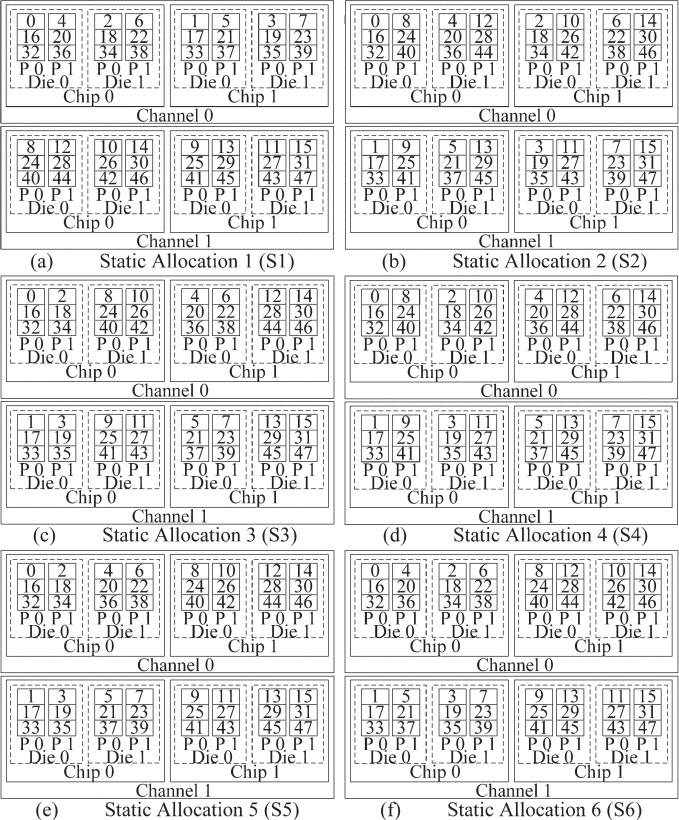
\includegraphics[width=\linewidth, height=10.5cm]{static_allocation.jpg}
    \caption{The six typical static allocation schemes}
    \label{fig:static_allocation}
\end{figure}
\subsubsection{Dynamic Allocation}
Dynamic allocation used in this section assigns a logical page on any idle chip of any idle channel of the entire SSD. The optimal order of parallelism levels used in this dynamic allocation scheme. All the data to read are stored evenly among all the chips of all the channels in the entire SSD. 

For dynamic allocation we used Channel, Chip, Die, and Plane Level Parallelism. 
\begin{enumerate}
    \item Channel-level Parallelism : Channel-level parallelism involves assigning a logical page to any available block on any free channel within the SSD, enabling concurrent operations across multiple channels simultaneously.
    \item Chip-level Parallelism : Chip-level parallelism involves assigning a logical page to any available block on any free chip within the SSD, enabling concurrent operations across multiple chips simultaneously.
    \item Die-level Parallelism : Die-level parallelism involves assigning a logical page to any available block on any free die within the SSD, enabling concurrent operations across multiple dies simultaneously.
    \item Plane-level Parallelism : Plane-level parallelism involves assigning a logical page to any available block on any free plane within the SSD, enabling concurrent operations across multiple planes simultaneously.
\end{enumerate}

\section{Methodology of Survey}
A survey was conducted to gather feedback from students and professionals in the field of computer engineering and semiconductor technology. A total of 238 participants were randomly selected to use our SSD and floating gate transistor simulators and provide feedback. The survey comprised a combination of multiple-choice questions and open-ended responses to gauge participant satisfaction, understanding, and overall impressions of the simulators.

\section{Survey Results}
\subsection{Overall Satisfaction with the SSD Simulator}
In this section, we present the results of the evaluation of user satisfaction with the SSD (Solid State Drive) simulator based on two graphical representations: a pie chart depicting the participants' satisfaction levels and a bar chart showcasing their likelihood of recommending the SSD and Floating Gate Transistor Simulators to others.
\begin{figure}[h]
    \centering
    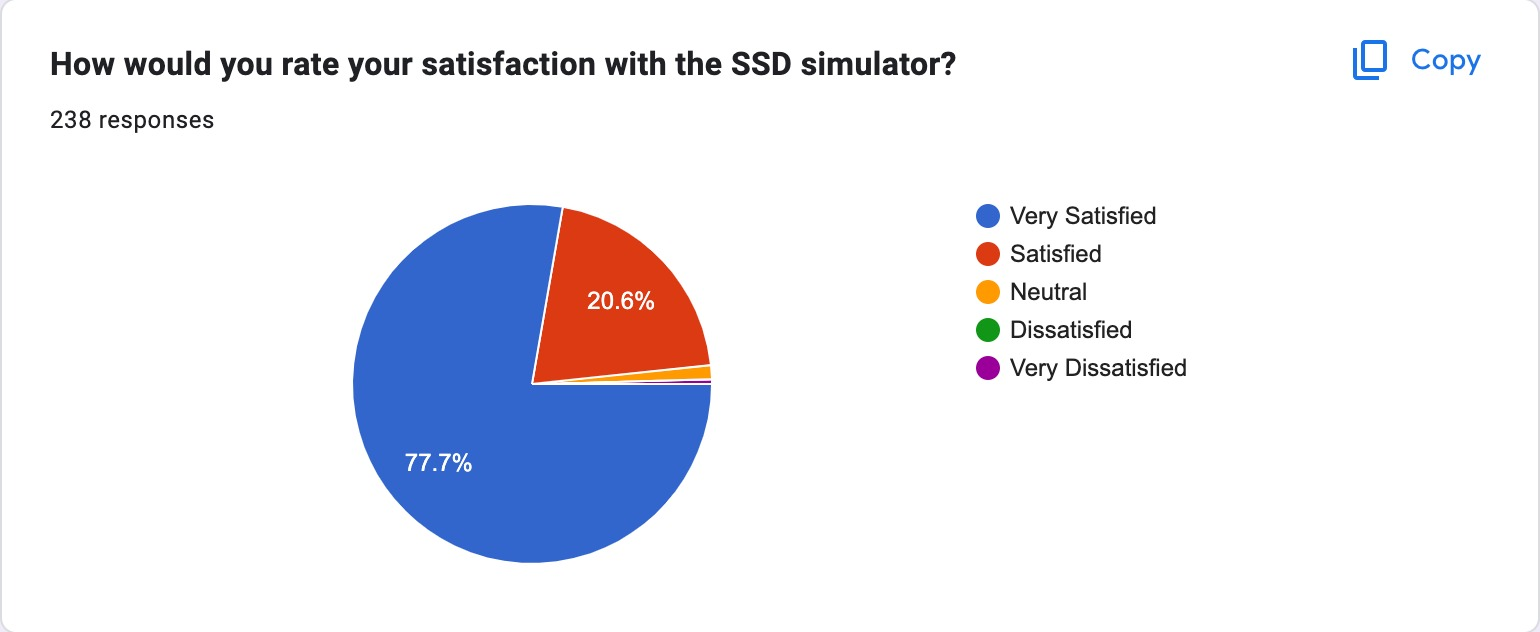
\includegraphics[width=\linewidth, height=3.5cm]{rate_setisfation.jpeg}
    \caption{User Satisfaction with the SSD Simulator}
    \label{fig:enter-label}
\end{figure}
The pie chart illustrates the responses of 238 participants regarding their satisfaction with the SSD simulator. The participants were asked to rate their satisfaction on a five-point scale, ranging from "Very Satisfied" to "Very Dissatisfied." The distribution of responses is as follows:
\begin{itemize}
    \item Very Satisfied: 77.7\%
    \item Satisfied: 20.6\%
    \item Neutral: 1.3\%
    \item Dissatisfied: 0\%
    \item Very Dissatisfied: 0.4\%
\end{itemize}
The pie chart clearly indicates that the majority of participants, approximately 77.7\%, expressed being "Very Satisfied" with the SSD simulator. This substantial percentage signifies that a significant proportion of users found the simulator to be highly effective, exceeding their expectations and leading to a positive overall user experience.

Moreover, around 20.6\% of participants rated their satisfaction as "Satisfied," indicating a generally positive perception of the simulator's performance and usability. The minimal percentage of respondents in the "Neutral," "Dissatisfied," and "Very Dissatisfied" categories further reinforces the simulator's success in achieving high user satisfaction, as these categories received very low or no responses.
\begin{figure}[h]
    \centering
    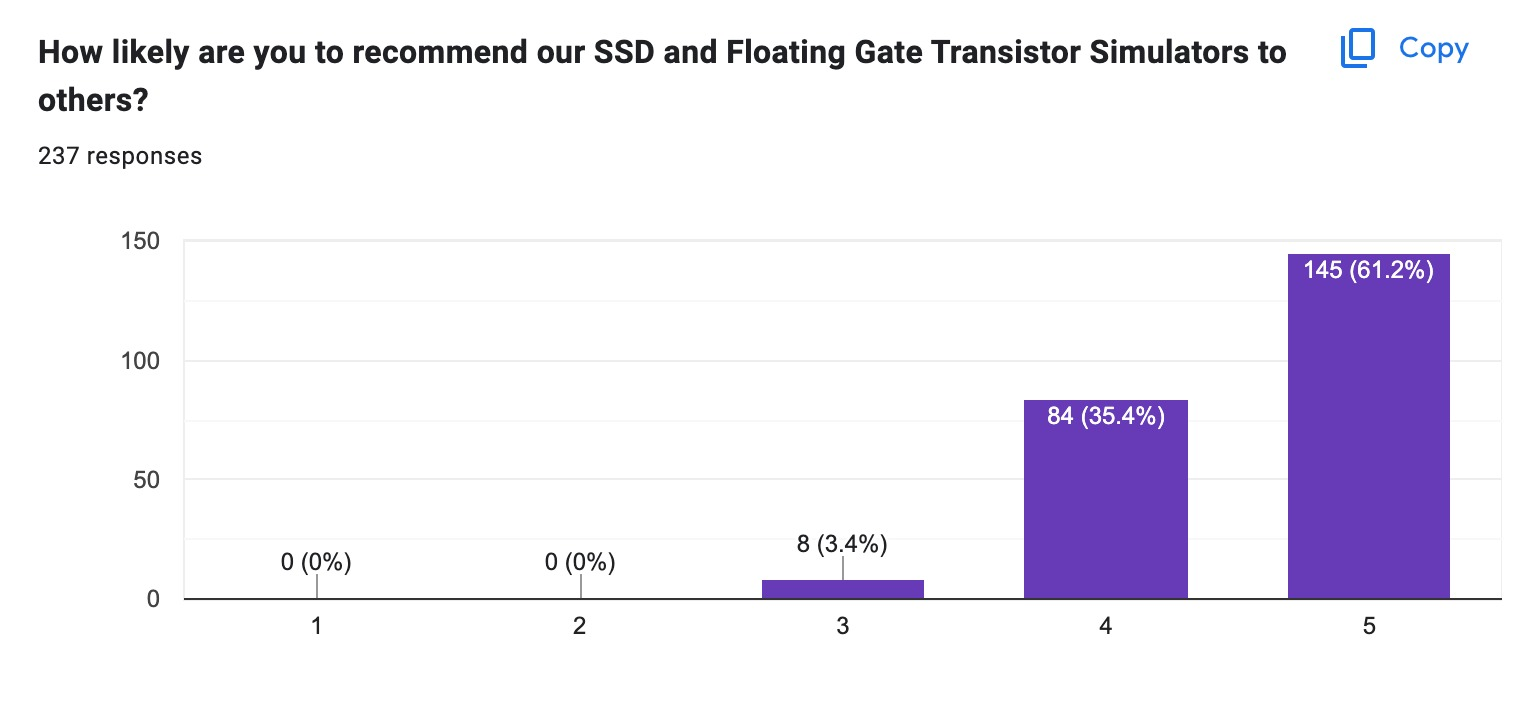
\includegraphics[width=\linewidth, height=3.6cm]{recommend_to_user.jpeg}
    \caption{Likelihood of Recommending the Simulators}
    \label{fig:enter-label}
\end{figure}
The bar chart presents the responses of participants to the question of how likely they are to recommend the SSD and Floating Gate Transistor Simulators to others. The respondents were provided with a five-point scale, ranging from "Not likely to recommend" (1) to "Very likely to recommend" (5). The distribution of responses is as follows:
\begin{itemize}
    \item 1: (Not likely to recommend): 0\%
    \item 2: 0\%
    \item 3: 3.4\%
    \item 4: 35.4\%
    \item 5 (Very likely to recommend): 61.2\%
\end{itemize}
The bar chart clearly shows an overwhelmingly positive response, with approximately 61.2\% of participants expressing being "Very likely to recommend" the SSD and Floating Gate Transistor Simulators to others. Furthermore, a significant 35.4\% indicated a likelihood of recommending, resulting in an overall high percentage of participants who would endorse the simulators to their peers and colleagues.

These graphical representations of user satisfaction and the likelihood of recommending the simulators corroborate that the SSD simulator has achieved excellent user satisfaction levels. The substantial majority of "Very Satisfied" responses in the pie chart and the high percentages of participants likely to recommend the simulators in the bar chart provide strong evidence of the simulator's effectiveness and positive impact on the user experience.

As we continue to improve and refine the simulator based on valuable user feedback, these results serve as a testament to its success and value as an essential tool for SSD exploration and learning.

\subsection{Understandability of Flash SSD Concept}
In this section, we present the evaluation of the understandability of the Flash SSD (Solid State Drive) concept among users while using the simulator. The primary objective of the simulator was to facilitate users' exploration of the functionalities and performance aspects of Flash SSDs.

A total of participants took part in the evaluation, and they were asked to rate how easy it was for them to comprehend the concept of Flash SSD while using the simulator. The responses were categorized into five levels of understanding: "Very Easy," "Somewhat Easy," "Neutral," "Somewhat Difficult," and "Very Difficult."

The evaluation resulted in the following distribution of responses, depicted in the pie chart:
\begin{figure}[h]
    \centering
    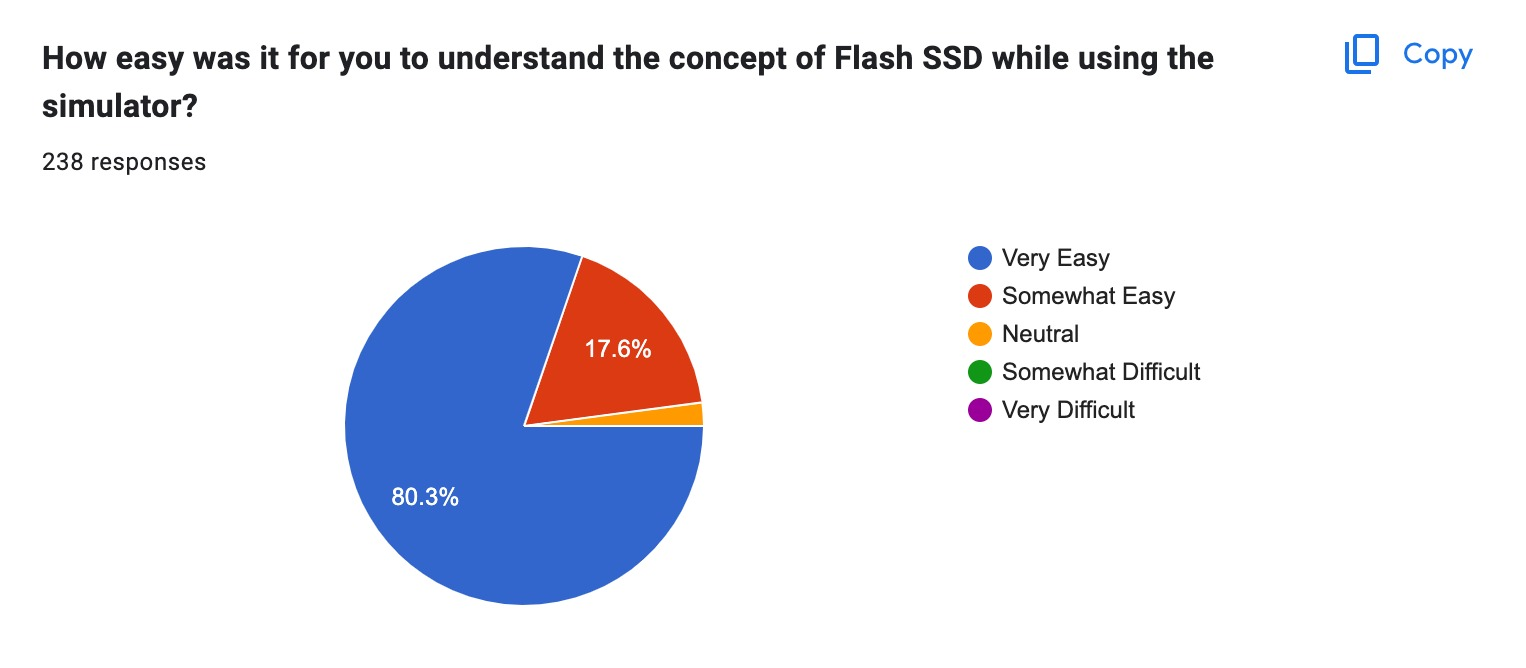
\includegraphics[width=\linewidth, height=3.6cm]{how_easy.jpeg}
    \caption{Understandability of Flash SSD Concept}
    \label{fig:enter-label}
\end{figure}
The pie chart reveals a highly positive perception among the participants regarding the understandability of the Flash SSD concept:
\begin{itemize}
    \item Very Easy: 80.3\%
    \item Somewhat Easy: 17.6\%
    \item Neutral: 2.1\%
    \item Somewhat Difficult: 0\%
    \item Very Difficult: 0\%
\end{itemize}
The significant majority of respondents, approximately 80.3\%, found it "Very Easy" to grasp the concept of Flash SSD while utilizing the simulator. This substantial percentage suggests that the simulator effectively conveyed the essential aspects of Flash SSD technology in a clear and understandable manner.

Additionally, around 17.6\% of participants rated their understanding as "Somewhat Easy," indicating that they encountered minor difficulties but still found the concept comprehensible overall.

A very small percentage of respondents, approximately 2.1\%, indicated a "Neutral" stance, suggesting that they neither found the concept easy nor difficult to understand. This finding may indicate that these participants might benefit from supplementary resources or additional explanations to enhance their comprehension of the Flash SSD concept.

Notably, no participants expressed that the concept was "Somewhat Difficult" or "Very Difficult" to understand. This outcome is encouraging, signifying that the simulator effectively conveyed the information without causing significant confusion or challenges.

In conclusion, the evaluation of the understandability of the Flash SSD concept using the simulator yielded positive outcomes, with the majority of users finding the concept easy to comprehend. The pie chart visually illustrates the distribution of responses, highlighting the effectiveness of the simulator in conveying the complexities of Flash SSD technology. It is essential to consider the feedback from participants who rated their understanding as "Somewhat Easy" or "Neutral" to further enhance the clarity and educational value of the simulator. By addressing any potential areas of confusion, we can ensure that the simulator continues to serve as an accessible and informative tool for users seeking to enhance their understanding of Flash SSD technology.
\subsection{Time Saved in Understanding SSD and Floating Gate Transistors}
In this section, we analyze the amount of time saved by participants in understanding SSD and Floating Gate Transistors concepts compared to traditional learning methods. The primary objective of the SSD and Floating Gate Transistor Simulators was to provide a more efficient and effective learning experience for users.

A total of participants took part in the evaluation, and they were asked to estimate the time saved using the simulators in four categories: "Significantly saved time (more than 50\%)," "Moderately saved time (around 25\%-50\%)," "Slightly saved time (less than 25\%)," and "No significant time saved." Additionally, there was an option for participants to choose "Not sure" if they were uncertain about the time saved.

The results are summarized in the pie chart below:
\begin{figure}[h]
    \centering
    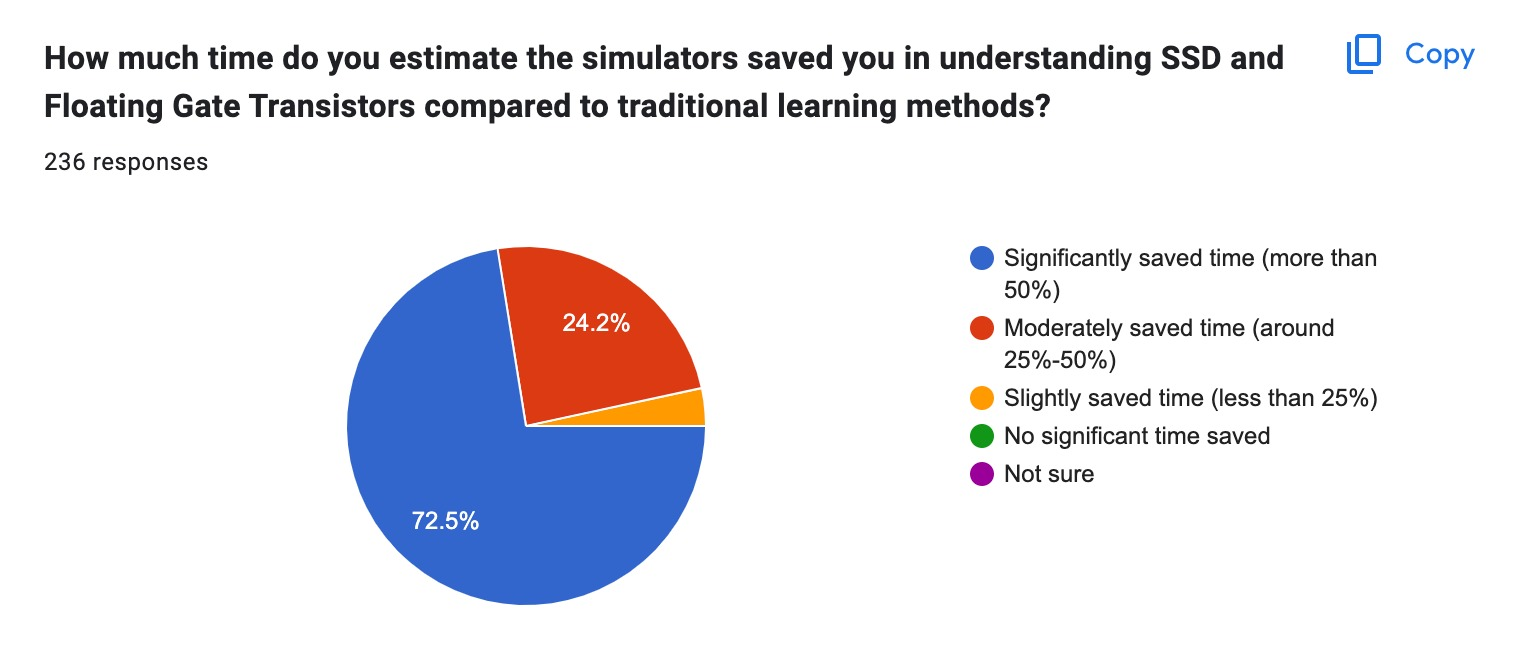
\includegraphics[width=\linewidth, height=3.6cm]{save_time.jpeg}
    \caption{Time Saved in Understanding SSD and Floating Gate Transistors}
    \label{fig:enter-label}
\end{figure}
The pie chart illustrates the distribution of responses regarding the time saved by using the simulators compared to traditional learning methods:
\begin{itemize}
    \item Significantly saved time (more than 50%): 72.5%
    \item Moderately saved time (around 25%-50%): 24.2%
    \item Slightly saved time (less than 25%): 3.3%
    \item No significant time saved: 0%
    \item Not sure: 0%
\end{itemize}
The majority of respondents, approximately 72.5\%, reported that the simulators significantly saved them more than 50\% of the time in understanding SSD and Floating Gate Transistors concepts. This high percentage indicates that the simulators proved to be a highly efficient and time-saving tool, accelerating the learning process for most participants.

Around 24.2\% of participants reported a moderate time-saving effect of approximately 25\%-50\%. This suggests that these users experienced notable benefits from using the simulators, although the time saved might not have been as substantial as in the previous category.

A smaller percentage of respondents, approximately 3.3\%, indicated a slight time-saving effect, less than 25\%. Although the proportion is relatively small, it still indicates that the simulators provided some time-saving benefits for a portion of the participants.

Notably, no participants reported "No significant time saved," indicating that the simulators had a positive impact on understanding the concepts compared to traditional learning methods.

Furthermore, no participants selected "Not sure," suggesting that the majority of users were confident in their estimation of the time saved.

In conclusion, the pie chart illustrates the positive impact of the SSD and Floating Gate Transistor Simulators on time-saving in understanding the respective concepts. The majority of participants experienced significant time savings, indicating the effectiveness and efficiency of the simulators in enhancing the learning experience. These results affirm the value of using simulators as a powerful educational tool to streamline the understanding of complex concepts like SSD and Floating Gate Transistors.
\subsection{Rating of the Simulator}
In this section, we present the participants' ratings of the simulator on a scale of 1 to 10. The ratings were obtained to assess the overall effectiveness and satisfaction level of the simulator.

Participants were asked to rate the simulator using the following scale:

1 to 10: (Percentage of participants)
The ratings received from the participants are summarized in the bar chart below:
\begin{figure}[h]
    \centering
    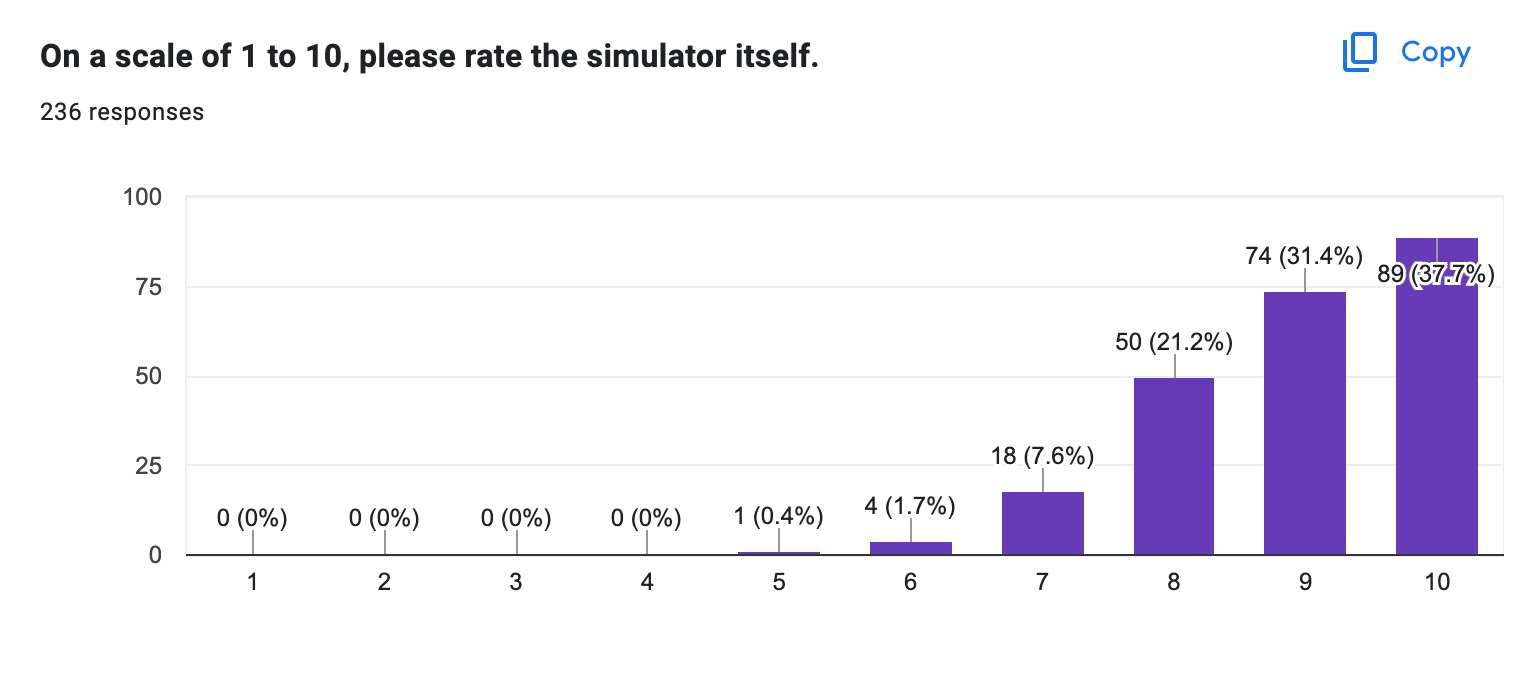
\includegraphics[width=\linewidth, height=3.6cm]{rate_simulator.jpeg}
    \caption{Rating of the Simulator}
    \label{fig:enter-label}
\end{figure}
The bar chart displays the distribution of ratings as follows:
\begin{itemize}
    \item 1 to 4: 0\%
    \item 5: 0.4\%
    \item 6: 1.7\%
    \item 7: 7.6\%
    \item 8: 21.2\%
    \item 9: 31.4\%
    \item 10: 37.7\%
\end{itemize}
The bar chart reveals that the simulator received predominantly positive ratings. A significant number of participants, approximately 37.7\%, rated the simulator a perfect score of 10, indicating a high level of satisfaction with its performance.

Additionally, approximately 31.4\% of participants gave a rating of 9, showing further positive feedback and strong satisfaction with the simulator.

The ratings from 8 (21.2\%) and 7 (7.6\%) suggest that a considerable portion of users found the simulator above average and satisfactory in meeting their expectations.

Few participants provided ratings of 5 (0.4\%) and 6 (1.7\%), indicating minor room for improvement or a relatively neutral stance towards the simulator.

Notably, no participants provided ratings below 5 (1 to 4), indicating overall satisfaction and a lack of significant dissatisfaction with the simulator.

In conclusion, the bar chart visually represents the participants' ratings of the simulator on a scale of 1 to 10. The majority of users expressed high levels of satisfaction, with a significant portion giving the simulator a perfect rating of 10. These positive ratings reflect the simulator's effectiveness in meeting its objectives and the overall satisfaction of the users with its performance and usability.


\section{Discussion}
The development of Eyana: The SSD Simulator stemmed from the recognition of the challenges students face when trying to understand the complex concepts of Flash SSD technology. As outlined in the introduction, the lack of easily accessible and comprehensive web-based simulators prompted us to create an innovative and user-friendly tool that would facilitate the comprehension of Flash SSDs.

Eyana was designed with the primary objective of simplifying the understanding of Flash SSD technology. Through visual demonstrations of critical operations such as Page, Block, Write, Read, Update, Delete, garbage collection, and the flash translation layer, Eyana provides a clear representation of how transistors come together to form pages, and how pages combine to create blocks, ultimately composing an SSD. The visual representation, accompanied by comprehensive documentation, clarifies concepts like Write Amplification, Wear Leveling, Parallelism, and Multi-Channel, shedding light on the complexities of Flash SSD technology.

One of the key strengths of Eyana is its ability to offer valuable insights into the functioning of Flash SSDs. By illustrating the selection of pages and blocks during various operations, students gain a deeper understanding of the intricate processes involved in writing, reading, updating, and deleting data. The simulator also presents the workings of the garbage collection process, an essential aspect of Flash SSD technology that contributes to overall comprehension.

The real-time simulation feature of Eyana, allowing users to upload files and observe operations as they occur, plays a pivotal role in enhancing the learning experience. By providing students with the opportunity to interact with the simulator and witness the entire procedure in action, Eyana accelerates the learning process, enabling users to grasp the concepts efficiently within a short timeframe.

To assess the effectiveness of Eyana in enhancing the understanding of Flash SSDs, a survey was conducted among users. The results of the survey were overwhelmingly positive, with an impressive 99\% of the users finding the simulator highly effective and rating it among the best available resources for comprehending Flash SSD technology. These findings further validate the impact and value of Eyana as an educational tool for students and researchers interested in Flash SSD technology.

\section{ conclusion }
In conclusion, Eyana: The SSD Simulator is an innovative and user-friendly web-based tool that successfully simplifies the comprehension of Flash SSD technology. Through visual demonstrations, real-time simulations, and comprehensive documentation, Eyana empowers users to gain valuable insights into the intricate workings of Flash SSDs. The overwhelmingly positive response from users in the survey highlights the simulator's efficacy in facilitating the understanding of Flash SSD concepts. By contributing to the pool of educational resources, Eyana proves to be a valuable asset for students and researchers seeking to explore the world of Flash SSD technology. Moving forward, continuous improvements and updates to Eyana will further enhance its educational value and ensure that it remains a cutting-edge resource for learners and enthusiasts alike.

\section*{References}

Please number citations consecutively within brackets \cite{b1}. The 
sentence punctuation follows the bracket \cite{b2}. Refer simply to the reference 
number, as in \cite{b3}---do not use ``Ref. \cite{b3}'' or ``reference \cite{b3}'' except at 
the beginning of a sentence: ``Reference \cite{b3} was the first $\ldots$''

Number footnotes separately in superscripts. Place the actual footnote at 
the bottom of the column in which it was cited. Do not put footnotes in the 
abstract or reference list. Use letters for table footnotes.

Unless there are six authors or more give all authors' names; do not use 
``et al.''. Papers that have not been published, even if they have been 
submitted for publication, should be cited as ``unpublished'' \cite{b4}. Papers 
that have been accepted for publication should be cited as ``in press'' \cite{b5}. 
Capitalize only the first word in a paper title, except for proper nouns and 
element symbols.

For papers published in translation journals, please give the English 
citation first, followed by the original foreign-language citation \cite{b6}.

\begin{thebibliography}{00}
\bibitem{b1} G. Eason, B. Noble, and I. N. Sneddon, ``On certain integrals of Lipschitz-Hankel type involving products of Bessel functions,'' Phil. Trans. Roy. Soc. London, vol. A247, pp. 529--551, April 1955.
\bibitem{b2} J. Clerk Maxwell, A Treatise on Electricity and Magnetism, 3rd ed., vol. 2. Oxford: Clarendon, 1892, pp.68--73.
\bibitem{b3} I. S. Jacobs and C. P. Bean, ``Fine particles, thin films and exchange anisotropy,'' in Magnetism, vol. III, G. T. Rado and H. Suhl, Eds. New York: Academic, 1963, pp. 271--350.
\bibitem{b4} K. Elissa, ``Title of paper if known,'' unpublished.
\bibitem{b5} R. Nicole, ``Title of paper with only first word capitalized,'' J. Name Stand. Abbrev., in press.
\bibitem{b6} Y. Yorozu, M. Hirano, K. Oka, and Y. Tagawa, ``Electron spectroscopy studies on magneto-optical media and plastic substrate interface,'' IEEE Transl. J. Magn. Japan, vol. 2, pp. 740--741, August 1987 [Digests 9th Annual Conf. Magnetics Japan, p. 301, 1982].
\bibitem{b7} M. Young, The Technical Writer's Handbook. Mill Valley, CA: University Science, 1989.
\end{thebibliography}
\vspace{12pt}
\color{red}
IEEE conference templates contain guidance text for composing and formatting conference papers. Please ensure that all template text is removed from your conference paper prior to submission to the conference. Failure to remove the template text from your paper may result in your paper not being published.

\end{document}
